\chapter{Propuesta de reconfiguración y predicción de errores en redes de distribución eléctrica}
\label{ch:fault_sg}

Partiendo de \gls{d2e} (Capítulo~\ref{ch:den2ne}), que establece las bases para mecanismos de control, esquemas de encaminamiento mediante etiquetado jerárquico y estrategias de gestión/planeamiento de recursos en entornos densos y heterogéneos, este capítulo explora su aplicación a la optimización y reconfiguración proactiva de redes de distribución eléctrica (\gls{sg}). La combinación de un mecanismo eficiente de descubrimiento/etiquetado con modelos de \gls{ml}/\gls{dl} permite abordar dos retos clave (Analizado en la Sección~\ref{subsubsec:propuestas_optimizacion}): (i) detectar y predecir anomalías o fallos antes de que afecten al servicio, y (ii) coordinar reconfiguraciones automáticas y seguras que minimicen pérdidas y aumenten la resiliencia del sistema.\\
\\
En este capítulo se presenta una propuesta novedosa que integra técnicas de aprendizaje automático (\gls{ml}), y aprendizaje profundo (\gls{dl}) para la predicción temprana de fallos en red con algoritmos de reconfiguración basados en el etiquetado jerárquico propuesto con \gls{d2e}. El sistema propuesto opera en tres capas: (a) adquisición y agregación de telemetría distribuida (sensores, medidores y nodos etiquetados), (b) motores predictivos de \gls{ml}/\gls{dl} que estiman la localización de fallos a corto plazo en la \gls{sg}, y (c) un módulo de decisión que traduce las predicciones en posibles acciones de reconfiguración.\\
\\
Este trabajo nació a raíz de \gls{d2e} (Carrascal \textit{et al.}~\cite{carrascal2024topology}), y se materializó como uno de los primeros TFM que pude dirigir en la universidad (Bartolomé \textit{et al.}~\cite{bartolome2024_smartgrids}), dando lugar a una propuesta (Carrascal \textit{et al.}~\cite{carrascal2024fault}) que pone de manifiesto la versatilidad y capacidad de \gls{d2e} para operar en diferentes dominios y casos de uso finales.

\section{Introducción}

Las \gls{sg} representan la solución futura para las redes de transmisión y distribución eléctrica~\cite{Vu1997,Amin2005}, cuyo objetivo principal es alcanzar una monitorización completa de la red que permita un mejor balance energético entre productores y consumidores. Uno de los aspectos más relevantes de las \gls{sg} es la reconfiguración de la distribución de energía dentro de la propia red. Esto resulta crucial porque permite reencaminar la potencia en caso de fallo en alguno de los enlaces de la red, o simplemente optimizar la distribución según un criterio determinado. Numerosas contribuciones existentes vistas en la Sección~\ref{subsubsec:propuestas_optimizacion} inciden especialmente en este último caso, en el que la reconfiguración mediante optimización reduce pérdidas por propagación o sobrecarga de línea, o actúa sobre otros parámetros eléctricos. De forma general, la mayoría de los algoritmos de reconfiguración aplicados a \gls{sg} que se centran en la resiliencia ante fallos buscan proporcionar rutas de respaldo o caminos alternativos para llevar a cabo la distribución. No obstante, las estrategias propuestas suelen ser siempre reactivas frente al fallo, ya sea de manera centralizada o distribuida.\\
\\
Por ello, en este trabajo nos proponemos generar una estrategia de reconfiguración preventiva, y por tanto proactiva, frente a fallos de red, aprovechando conjuntos de datos reales de \gls{sg} y técnicas de \gls{ml} y \gls{dl}. Como se ha indicado, el enfoque propuesto descansa sobre \gls{d2e}~\cite{carrascal2024topology}. Partimos de dicha base para desarrollar un mecanismo de predicción de fallos que clasifica rutas alternativas obtenidas en la etapa de etiquetado jerárquico suministrado por \gls{d2e}, con el fin de identificar de forma anticipada aquellas con mayor probabilidad de provocar errores en la red. Existen múltiples criterios en las \gls{sg} que pueden dar lugar a fallos en la red, en nuestro caso, analizaremos cuando una línea de la red excede la capacidad física de la misma. En consecuencia, tras el análisis del estado del arte (Sección~\ref{subsubsec:conclu_opt}), las principales aportaciones de nuestro trabajo son las siguientes:

\begin{enumerate}
    \item Una solución de predicción de fallos específicamente orientada a la reconfiguración de \gls{sg}, entrenada y validada con conjuntos de datos reales tal y como se detalla en la Sección~\ref{sec:Faultdatasets}.

    \item Generalizable a topologías de cualquier tipo, forma o tamaño, evaluada con el generador de topologías aleatorias \gls{brite} y parámetros realistas, empleando parámetros inspirados en el modelo \gls{ieee} 123 Node Test Feeder~\cite{Schneider17}. A partir de estas validaciones, hemos estudiado la optimización de varios modelos de \gls{ml} y \gls{dl} para \gls{d2e} mediante selección de características y evaluación del modelo predictivo más adecuado para cada escenario.
\end{enumerate}

Este último punto es de especial interés, dado que, en la literatura revisada, la mayoría de propuestas que emplean \gls{ai}/\gls{ml} suelen tender a generar modelos con un único propósito y un único tipo de red, no siendo extrapolables a otros tipos/casuísticas de \gls{sg}.




\section{Búsqueda y análisis de fuentes de datos}
\label{sec:Faultdatasets}


Para evaluar de manera integral las diferentes técnicas de \gls{ai} aplicadas a la predicción de fallos en escenarios de reconfiguración de \glspl{sg}, resulta esencial disponer de un conjunto de datos de alta calidad. Tanto la calidad como la cantidad de datos son factores determinantes para definir un modelo consistente. En el contexto energético, nuestra experiencia demuestra que existe una menor disponibilidad de conjuntos de datos. La protección de la privacidad de los usuarios en la medición y análisis de su comportamiento energético reduce el número de datasets públicos disponibles, ya que estos dependen principalmente de las compañías eléctricas~\cite{powercons}.\\
\\
No obstante, la búsqueda de la optimización en la distribución de la energía y la reducción del consumo de los usuarios, junto con otras motivaciones medioambientales, ha favorecido la creación de conjuntos de datos públicos en los últimos años. La Tabla~\ref{tab:faultdatasets} muestra varios datasets residenciales analizados, junto con detalles sobre su implementación, tales como la localización, el número de viviendas, el periodo de despliegue, la frecuencia de muestreo y los parámetros eléctricos medidos. Como parte de nuestro análisis, y con el objetivo de evaluar y seleccionar el dataset más adecuado entre los disponibles en la Tabla~\ref{tab:faultdatasets}, se han considerado los siguientes requisitos:


\begin{itemize}
    \item \textbf{Cantidad}: Es fundamental revisar la cantidad de datos disponibles en cada dataset, asegurando que incluyan mediciones de un número amplio de viviendas y que abarquen periodos prolongados de tiempo para analizar de manera efectiva los patrones de consumo energético.

    \item \textbf{Calidad}: La calidad de los datos depende de la resolución de las mediciones. Datasets como \textit{REDD} y \textit{BLUED} ofrecen frecuencias de muestreo elevadas, lo que permite una mejor desagregación del consumo energético y un análisis más representativo del comportamiento energético.
    
    \item \textbf{Localización}: La localización de los datos es relevante, ya que influye en las diferencias de voltaje entre países. Por ejemplo, datasets de Estados Unidos, como \textit{BLUED}, operan a menos de 120V, mientras que conjuntos europeos como \textit{ECO} trabajan hasta 230V.
    
    \item \textbf{Parametrización}: Las muestras incluyen tensión (V), corriente (I) y potencia (tanto la activa (P), la reactiva (Q), y la aparente (S)), cada una asociada a una marca temporal y un identificador correspondiente a la vivienda. Algunos datasets, como \textit{HUE} y \textit{SustDataED}, también incorporan datos ambientales, lo cual resulta relevante para comprender el impacto de las condiciones climáticas con la generación de potencia renovable.
    
    \item \textbf{Generación Fotovoltaica}: En el contexto de las \glspl{sg}, es esencial elegir conjuntos de datos que incluyan información sobre generación de energía renovable, como \textit{Smart*} y \textit{SustDataED}.
\end{itemize}

Entre los datasets analizados, se seleccionó especialmente \textit{SustDataED}, debido al elevado número de usuarios con perfiles tanto de consumo, como de producción a lo largo de un periodo extenso de tiempo. Asimismo, resulta clave que las muestras presenten una buena resolución y que ofrezcan información en tiempo real sobre las condiciones climáticas de la ubicación en la que se encuentran las viviendas. En las siguientes secciones, se examina en detalle este conjunto de datos y se describen los principales criterios de diseño aplicados para generar el dataset final, elaborado a partir de \textit{SustDataED} y complementado con la herramienta PVWatts, que finalmente se utilizó en nuestra evaluación.

\begin{sidewaystable}
    \centering
     % o \scriptsize si quieres reducir aún más la fuente
    \begin{tabularx}{\textheight}{|l|X|c|c|c|c|}
        \hline
        \textbf{Nombre} & \textbf{Localización} & \textbf{Residencias} & \textbf{Periodo (días)} & \textbf{Resolución} & \textbf{Parámetros} \\ \hline
        \textit{AMPds2} \cite{ampds2} & Vancouver (Canadá) & 1 & 730 & 60s & I, V, P, S, F, pf \\ \hline
        \textit{BLUED} \cite{blued} & Pittsburgh (EE.\,UU.) & 1 & 8 & 83.33$\mu$s & I, V, eventos switch \\ \hline
        \textit{ECO} \cite{eco} & Suiza & 6 & 244 & 1s & P \\ \hline
        \textit{GREEND} \cite{greend} & Italia y Austria & 9 & 310 & 1s & P \\ \hline
        \textit{HUE} \cite{hue} & Columbia Británica (Canadá) & 28 & 60 & 1s & P \\ \hline
        \textit{iAWE} \cite{iawe} & Nueva Delhi (India) & 1 & 73 & 1s & V, I, P, S \\ \hline
        \textit{REDD} \cite{redd} & Boston (EE.\,UU.) & 6 & 119 & 66.66$\mu$s & I, V, P \\ \hline
        \textit{Smart*} \cite{smart*} & Massachusetts (EE.\,UU.) & 3 & 90 & 60s & P, S, V, I \\ \hline
        \textit{SustDataED} \cite{sustdata} & Madeira (Portugal) & 50 & 1144 & 60s & I, V, P, Q, S \\ \hline
        \textit{UK-DALE} \cite{ukdale} & Reino Unido & 5 & 499 & 62.5$\mu$s & P, estados de switch \\ \hline
    \end{tabularx}
    \caption{Comparación de datasets sobre el consumo público de energía eléctrica.}
    \label{tab:faultdatasets}
\end{sidewaystable}

\subsection{Análisis del dataset - SustDataED}

El dataset \textit{SustDataED}~\cite{sustdata} fue creado como parte del proyecto de investigación SINAIS, cuyo objetivo es proporcionar retroalimentación ecológica a los usuarios para fomentar un comportamiento energético sostenible y un mayor uso de fuentes de energía renovable. Este dataset abarca cinco años de datos de consumo y producción energética de 50 hogares en la ciudad de Funchal (Madeira, Portugal), divididos en tres despliegues diferentes. Esto implica que no existen mediciones de los 50 hogares de forma simultánea a lo largo de los cinco años del proyecto, sino agrupadas en tres conjuntos separados. La Figura~\ref{fig:demographics} muestra los tres despliegues mencionados. Dado que trabajamos con mediciones de consumo y generación que están parcialmente correlacionadas con condiciones meteorológicas y temporales, seleccionaremos el periodo de tiempo con el mayor número de hogares desplegados simultáneamente. En nuestro caso, se elige el primer despliegue, en el cual se dispone de mediciones de hasta 23 hogares de manera simultánea.
 

\begin{figure}[ht!]
    \centering
    \includegraphics[width=\textwidth]{fig/06_fault_sg/fault_sg_01.pdf}
    \caption{Series temporales de los diferentes despliegues del dataset \textit{SustDataED}.}
    \label{fig:demographics}
\end{figure}

Los datos disponibles en \textit{SustDataED} son bastante variados. La Tabla~\ref{tab:SustDataEDMeasurements} muestra los diferentes tipos de mediciones incluidos en el dataset. Sin embargo, no todas ellas son relevantes para este estudio. Por ejemplo, un alto nivel de granularidad, como las mediciones de eventos de potencia o de eventos de usuario, no es necesario para nuestro análisis. Como se observa en la Tabla~\ref{tab:SustDataEDMeasurements}, las mediciones relacionadas con la producción de energía presentan cierta incertidumbre. A primera vista, \textit{SustDataED} resulta adecuado porque ofrece mediciones reales de producción fotovoltaica. No obstante, estos datos se reportan como valores agregados y corresponden a un sistema fotovoltaico que abastece a todos los hogares del despliegue, sin especificar información sobre las dimensiones del sistema. Además, no está claro si el tamaño del sistema fotovoltaico aumenta con el tiempo, lo que dificulta el análisis a nivel individual de cada hogar.


\begin{table}[ht!]
\centering
%\resizebox{0.6\textwidth}{!}{%
\begin{tabular}{|l|c|}
\hline
\textbf{Tipo de medida}                       & \textbf{Utilidad} \\ \hline
Mediciones del consumo energético                    & \checkmark             \\ \hline
Mediciones de la producción de energía                    & \textbf{?}             \\ \hline
Mediciones demográficas                           & \checkmark              \\ \hline
Mediciones de las condiciones ambientales y climáticas & \checkmark              \\ \hline
Mediciones de eventos de usuario                           & \text{\sffamily X}             \\ \hline
Mediciones de eventos de potencia                         & \text{\sffamily X}               \\ \hline
\end{tabular}%
%}
\caption{Tipos de mediciones en el dataset \textit{SustDataED}.}
\label{tab:SustDataEDMeasurements}
\end{table}


\subsection{Deficiencias del dataset - SustDataED}

Dado que la literatura sobre \textit{SustDataED} no ofrecía claridad en cuanto a las mediciones de producción de energía fotovoltaica a nivel de individual de cada hogar, se buscó una alternativa para conformar un nuevo conjunto de datos de producción. Por ello, se propuso llevar a cabo simulaciones de producción fotovoltaica en la ciudad de Funchal, con las características y dimensiones de un sistema fotovoltaico convencional, para así tener una estimación coherente de la generación a nivel de un hogar. Para realizar esta simulación de datos de producción, se eligieron dos herramientas con el fin de comparar y garantizar que los resultados obtenidos fueran consistentes:


\begin{itemize}
    \item \textbf{Global Solar Atlas}~\cite{globalsolar}: Esta plataforma está financiada por el Programa de Asistencia para la Gestión del Sector Energético (ESMAP), con el objetivo de mapear los recursos de energía renovable a nivel mundial, proporcionando acceso tanto a datos promediados a largo plazo como a datos en tiempo real para cualquier ubicación del planeta.

    \item \textbf{PVWatts}~\cite{pvwatts}: Esta plataforma es proporcionada por el Laboratorio Nacional de Energías Renovables (NREL), que forma parte del Departamento de Energía de los Estados Unidos.

\end{itemize}

Para cada herramienta, la ubicación se fijó en Funchal (Portugal), dado que el análisis debe corresponder a los datos recogidos en el conjunto \textit{SustDataED}. Una vez establecida la localización, se configuró el sistema fotovoltaico para cada hogar y se extrajeron las capas de datos relevantes, como el \gls{dni} ($\frac{kWh}{m^{2}}$) y el \gls{pvout} ($\frac{kWh}{kWp}$), que son parámetros clave para estimar la producción de los sistemas fotovoltaicos. \\
\\
Además, los factores climáticos desempeñan un papel crucial en la verificación de la consistencia de la energía generada. Según las clasificaciones climáticas de Köppen y Trewartha, Funchal presenta un clima mediterráneo con influencias oceánicas, o bien un clima templado con veranos secos. Al estar situada en una zona subtropical, la ciudad experimenta variaciones diarias mínimas de temperatura, lo que se traduce en condiciones relativamente estables a lo largo del año.\\
\\
Tras configurar ambos sistemas, se alinearon las fechas correspondientes a las series temporales de \textit{SustDataED} para recopilar los datos de producción fotovoltaica. En ambas herramientas, tal como se muestra en la Figura~\ref{fig:DNIpvoutVS}, se llevó a cabo un análisis comparativo de los mismos parámetros, \gls{dni} y \gls{pvout}, durante los mismos periodos de tiempo. Los resultados, ilustrados en la Figura~\ref{fig:DNIpvoutVS}, resultaron ser prácticamente idénticos. Una vez verificada esta consistencia entre las dos herramientas para la simulación de valores de producción fotovoltaica, se seleccionó \textit{PVWatts} debido a sus capacidad de exportar datos de forma más sencilla, lo que facilitó la integración con los datos de \textit{SustDataED} para la construcción del dataset final.

\begin{figure}[ht!]
    \centering
    \begin{minipage}{0.47\textwidth}
        \centering
        \includegraphics[width=\linewidth]{fig/06_fault_sg/fault_sg_02a.pdf}
        \subcaption{\textit{Global Solar Atlas} - DNI}
    \end{minipage}
    \hfill
    \begin{minipage}{0.47\textwidth}
        \centering
        \includegraphics[width=\linewidth]{fig/06_fault_sg/fault_sg_02b.pdf}
        \subcaption{\textit{Global Solar Atlas} - PVOUT}
    \end{minipage}
    
    \vspace{0.5cm} % Espacio entre filas
    
    \begin{minipage}{0.47\textwidth}
        \centering
        \includegraphics[width=\linewidth]{fig/06_fault_sg/fault_sg_02c.pdf}
        \subcaption{\textit{PVWatts} - DNI}
    \end{minipage}
    \hfill
    \begin{minipage}{0.47\textwidth}
        \centering
        \includegraphics[width=\linewidth]{fig/06_fault_sg/fault_sg_02d.pdf}
        \subcaption{\textit{PVWatts} - PVOUT}
    \end{minipage}
    
    \caption{Comparación entre \textit{Global Solar Atlas} y \textit{PVWatts}, valores mensuales totales de producción de energía fotovoltaica (PVOUT) frente a la irradiación directa normal (DNI).}
    \label{fig:DNIpvoutVS}
\end{figure}

Además, se realizó un análisis de correlación exhaustivo sobre los parámetros de generación de energía fotovoltaica tanto del conjunto de datos \textit{SustDataED} como de \textit{PVWatts}, con el objetivo de evaluar de forma concluyente la fiabilidad de los datos de producción energética. Al examinar la correlación entre las variables climáticas y la generación de energía en ambos conjuntos de datos, tal como se muestra en la Figura~\ref{fig:corrSUST_PVWATTS}, emergen patrones diferenciados.\\
\\
Para \textit{SustDataED} (Figura~\ref{fig:corrSUST_PVWATTS} (a)), es evidente que la temperatura presenta una correlación débil con la potencia generada, arrojando un coeficiente de tan solo 0.279. Esta falta de correlación significativa se repite en otras variables, lo que dificulta el análisis de la producción de energía en relación con las condiciones climáticas. En contraste, para el conjunto de datos \textit{PVWatts} (Figura~\ref{fig:corrSUST_PVWATTS} (b)), la mayoría de los parámetros muestran un alto grado de correlación, cercano a la unidad. Por ejemplo, la correlación entre la irradiancia del plano del array, que es la cantidad total de radiación solar que incide sobre la superficie de un panel solar, y la generación de potencia es prácticamente ideal, con un coeficiente de 0.999, como se observa claramente en la gráfica.


\begin{figure}[ht!]
    \centering
    \begin{minipage}{0.39\textwidth}
        \centering
        \includegraphics[width=\linewidth]{fig/06_fault_sg/fault_sg_03a.pdf}
        \subcaption{Parámetros fotovoltaicos - \textit{SustDataED}}
    \end{minipage}
    \hfill
    \begin{minipage}{0.54\textwidth}
        \centering
        \includegraphics[width=\linewidth]{fig/06_fault_sg/fault_sg_03b.png}
        \subcaption{Parámetros fotovoltaicos - \textit{PVWatts}}
    \end{minipage}

    \caption{Comparación mediante matrices de correlación de los parámetros de producción fotovoltaica.}
    \label{fig:corrSUST_PVWATTS}
\end{figure}

\begin{figure}[ht!]
    \centering
    \includegraphics[width=\linewidth]{fig/06_fault_sg/fault_sg_04.pdf}
    \caption{Patrones de correlación entre los parámetros de producción en \textit{PVWatts}.}
    \label{fig:corrUST_PVWATTS_graphs}
\end{figure}

Como se ilustra en la Figura~\ref{fig:corrUST_PVWATTS_graphs}, el diagrama de dispersión correspondiente a la correlación de los parámetros de producción de \textit{PVWatts}, revela que los parámetros más significativos para la generación de energía fotovoltaica son: la irradiancia del plano del array del panel solar y la temperatura de las celdas solares. Dadas las limitaciones de los datos de producción de \textit{SustDataED}, especialmente en términos de precisión y granularidad, se decidió utilizar los datos de producción simulados mediante la herramienta \textit{PVWatts}. Esta elección se sustenta en la consistencia mostrada por los datos de \textit{PVWatts} al compararlos con los resultados del \textit{Global Solar Atlas}, y la capacidad que tiene la herramienta para exportar datos de simulación para la integración de los datos de generación fotovoltaica en el dataset final. En la siguiente sección, se presentará el dataset final, sus características clave, y la organización de los ficheros resultantes. 

\subsection{Dataset final}
\label{subsec:keymondata}
Tras identificar y abordar las limitaciones de \textit{SustDataED} mediante la incorporación de la herramienta \textit{PVWatts} para los datos de generación fotovoltaica, se procesó el conjunto completo de datos con el fin de crear el dataset final. El flujo de procesamiento de datos se muestra en la Figura~\ref{fig:dataprocessing}. Como se observa, existen dos ramas principales: la primera procede del conjunto \textit{SustDataED} e incluye todos los datos de consumo de los hogares, mientras que la segunda corresponde a los datos de generación fotovoltaica. De los 50 hogares, solo se seleccionaron 23 pertenecientes al primer despliegue, como se indicó previamente. Posteriormente, se generaron 23 perfiles de generación fotovoltaica, conformando finalmente 23 archivos de cargas netas reales, que representan la suma de consumo y generación. Los campos finales incluidos en el dataset final se detallan en la Tabla~\ref{tab:datacombinacion}.

\begin{table}[H]
  \centering
  \resizebox{\textwidth}{!}{  
  \begin{tabular}{|c|c|c|}
  \hline
  \multicolumn{1}{|c|}{\textbf{Campo}} & \multicolumn{1}{c|}{\textbf{Descripción}} & \textbf{Unidades} \\ \hline
  \textit{timestamp} & Instante temporal de medida & datetime \\ \hline
  \textit{datetime} & Fecha del valor promedio & datetime \\ \hline
  \textit{H} & Hora del valor promedio & - \\ \hline
  \textit{iid} & Identificador de vivienda & - \\ \hline
  \textit{Diffuse Irradiance} & Índice de radiación difusa (DIF) & W/m2 \\ \hline
  \textit{Plane of Array Irradiance} & Índice de radiación en el plano del array (POA) & W/m2 \\ \hline 
  \textit{Ambient Temperature} & Temperatura ambiente & C \\ \hline
  \textit{Cell Temperature} & Temperatura de las células solares & C \\ \hline
  \textit{DC Array Output} & Potencia de salida DC del array & W \\ \hline
  \textit{AC System Output} & Potencia de salida AC del sistema & W \\ \hline
  \textit{Pavg} & Potencia consumida & W \\ \hline
  \textit{Dif} & Carga neta calculada & W \\ \hline
  \end{tabular}
  }
  \caption{Características principales del dataset final (\textit{KeyMonData}).}
  \label{tab:datacombinacion}
\end{table}

\begin{sidewaysfigure}
    \centering
    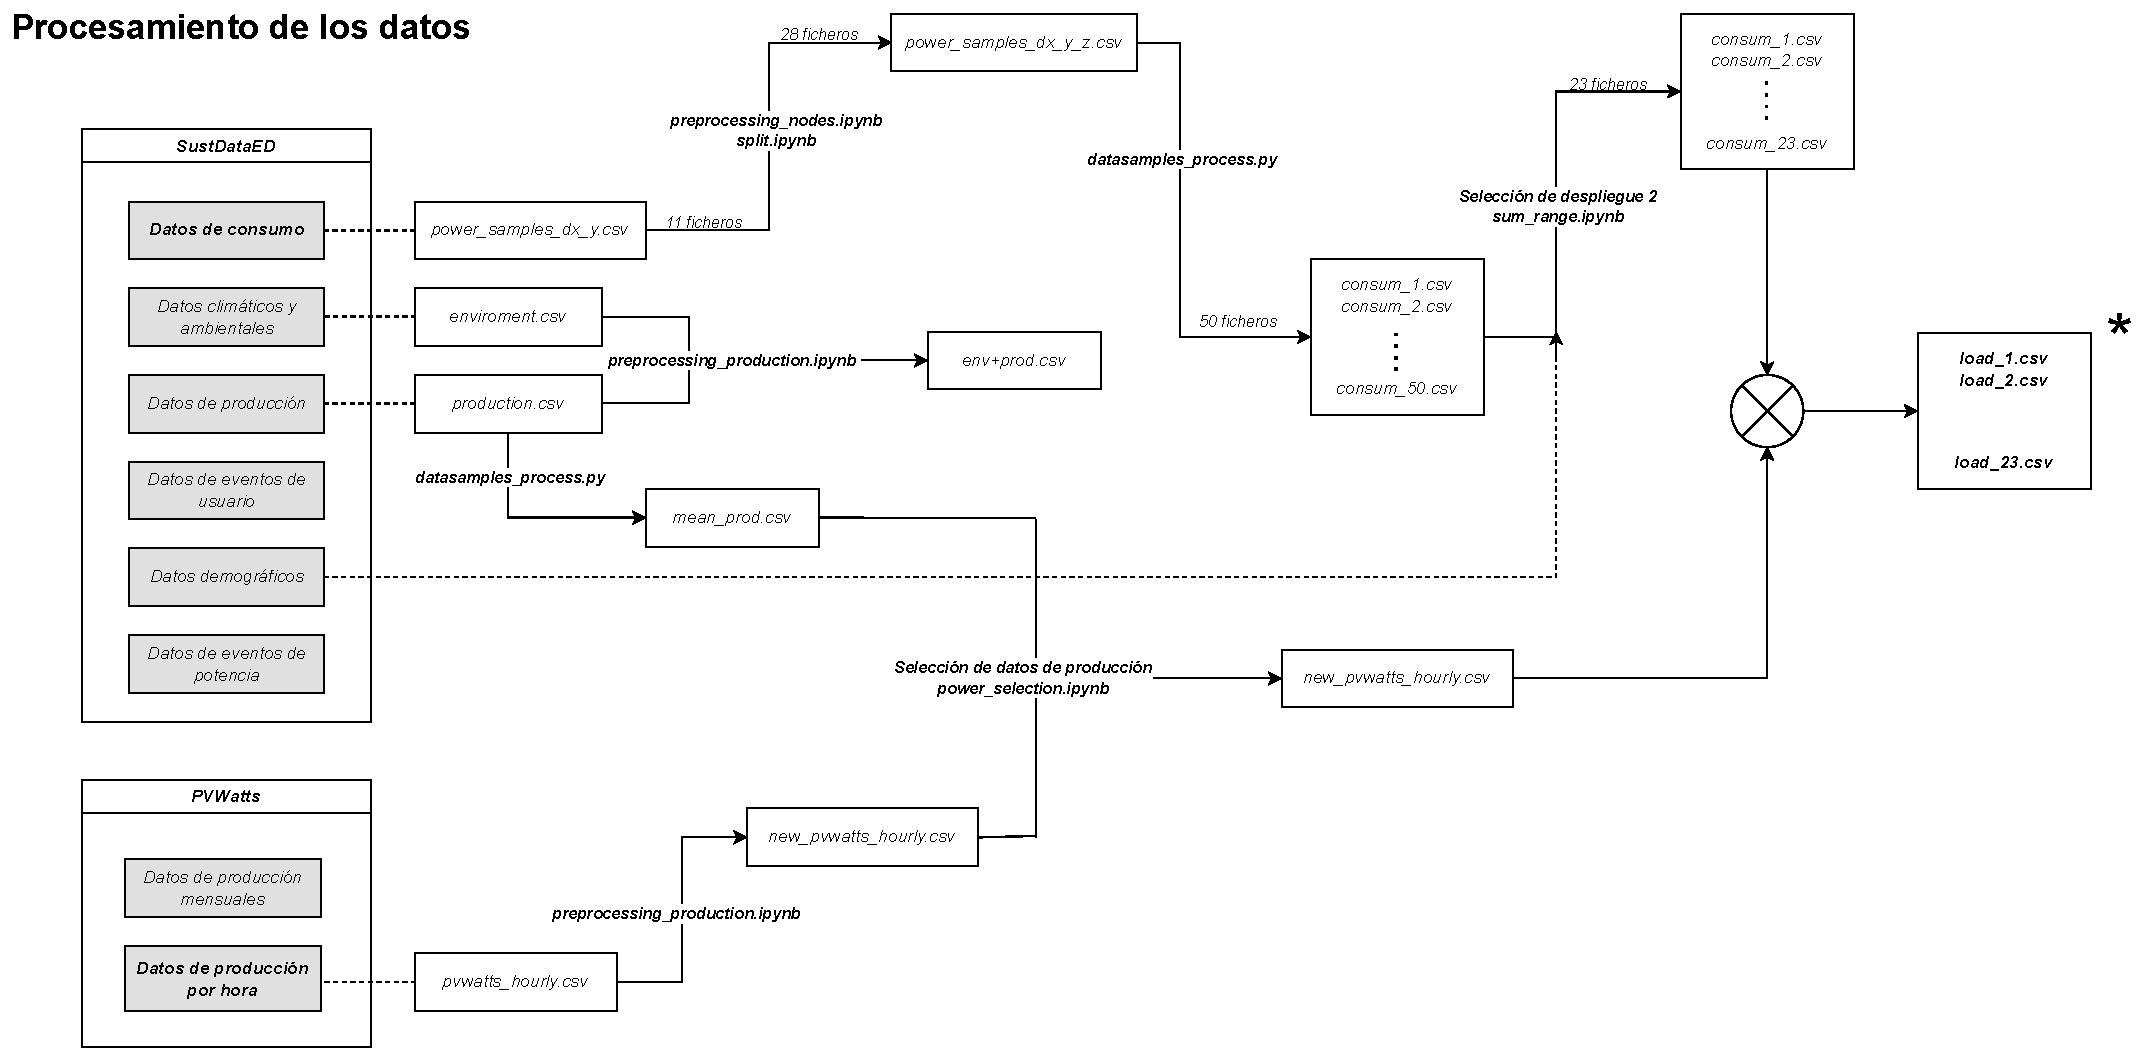
\includegraphics[width=\textwidth]{fig/06_fault_sg/fault_sg_05.drawio.pdf}
    \caption{Esquema de procesamiento de datos para la generación del dataset final.}
    \label{fig:dataprocessing}
\end{sidewaysfigure}

Este nuevo conjunto de datos requirió un procesamiento adicional para limitar tanto su tamaño como la serie temporal, de modo que se ajustara al despliegue especificado. Además, para hacerlo más manejable, los datos fueron sintetizados. Concretamente, \textit{SustDataED} ofrece medidas con una resolución a nivel de minuto; sin embargo, trabajar con muestras minuto a minuto resulta innecesario, dado que las variaciones de consumo son mínimas. Por ello, se redujo la resolución a muestras horarias. Así, si el primer despliegue se restringe a un año de duración, se obtienen 8760 intervalos temporales ($24\: h \times 365\: dias$) por cada hogar, para un total de 23 hogares.\\
\\
En cuanto a la convención de nombres de archivos, cada fichero fue etiquetado como \textit{load\_x.csv}, donde $x$ corresponde al identificador del hogar para las cargas calculadas. En consecuencia, se generaron un total de 23 archivos de cargas (\textit{load\_x.csv}), cada uno con 8760 intervalos temporales. Tras el procesamiento, limpieza y síntesis, el nuevo dataset fue denominado \textit{KeyMonData} y se ha puesto a disposición pública para su uso por parte de cualquier interesado~\cite{paulaTFM}.



\section{Algoritmo de reconfiguración y propuesta de extensión}  

El algoritmo de reconfiguración para las \gls{sg}, sobre el cual se construirán los modelos de \gls{ml} y \gls{dl}, es \gls{d2e}~\cite{carrascal2024topology}. Como se ha explicado anteriormente, ver Capítulo~\ref{ch:den2ne}, \gls{d2e} es un algoritmo diseñado para el descubrimiento de rutas en redes densas y heterogéneas, permitiendo automatizar el proceso de encaminamiento desde los nodos hoja hasta el nodo raíz de la topología, al tiempo que gestiona de forma eficiente el uso compartido de recursos. En el contexto específico de una \gls{sg}, el nodo raíz se define como aquel que dispone de conexión directa con la red de distribución eléctrica, mientras que los nodos ``hoja'' representan el resto de nodos de la \gls{sg}. \\
\\
Para explicar con mayor detalle el proceso de reconfiguración seguido por \gls{d2e}, la Figura~\ref{fig:load_power_balancing} ilustra un escenario de redistribución de carga dentro de una \gls{sg}, similar al ejemplo de la topología \gls{ieee} 5-bus. En verde se muestran los nodos con superávit de carga, que puede ser ofrecida a otros nodos de la red. En naranja se destacan los nodos que demandan energía de sus vecinos o, en última instancia, del nodo raíz. Sin embargo, calcular todas las posibles soluciones de redistribución de carga puede ser computacionalmente complejo en un tiempo razonable. Por ejemplo, la Figura~\ref{fig:load_power_balancing} (a) muestra una redistribución subóptima de recursos, que ocurre cuando los vecinos toman decisiones locales, lo que lleva a que la mayoría de solicitudes se dirijan al nodo con un superávit de +100 (insuficiente para cubrir toda la demanda). En cambio, la Figura~\ref{fig:load_power_balancing} (b) representa un escenario de distribución óptima, que requiere un enfoque más sofisticado para la distribución eficiente de recursos.


\begin{figure}[H]
    \centering
    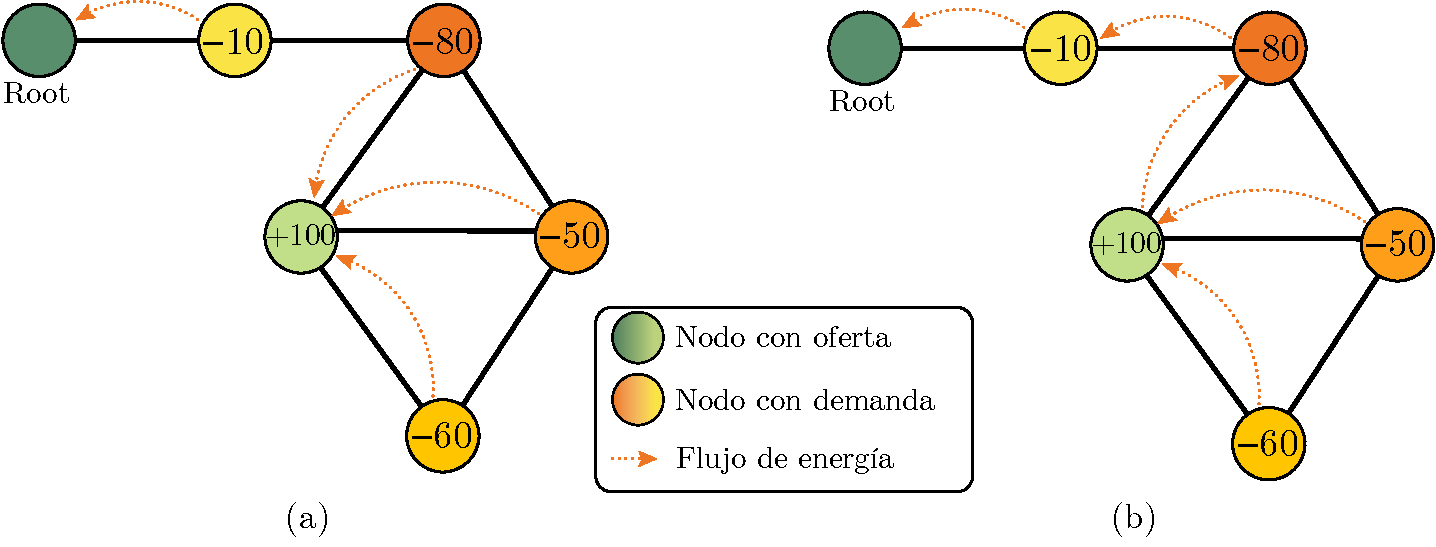
\includegraphics[width=0.9\linewidth]{fig/06_fault_sg/fault_sg_06.pdf}
    \caption{Ejemplo de redistribución de carga en una SG.}
    \label{fig:load_power_balancing}
\end{figure}

Para abordar este problema en las \gls{sg}, \gls{d2e} propone una solución en tres fases. La primera fase, mostrada en la Figura~\ref{fig:labelspropagation}, consiste en explorar todas las rutas posibles desde el nodo raíz hasta cada nodo de la topología (mecanismo similar al visto en la Sección~\ref{subsec:fase1}). Esta exploración, como se ilustra en la figura, se realiza mediante el uso de etiquetas. El proceso comienza en el nodo raíz, que genera la primera etiqueta (\textit{1}) y la transmite a todos sus vecinos inmediatos, en este caso al nodo 2. El nodo 2 recibe la etiqueta, añade su identificador de nodo, la almacena en su tabla de aprendizaje y, a continuación, la transmite de manera similar a todos sus vecinos contiguos. De esta forma, el nodo 3 recibe la etiqueta \textit{1.2}, lo que indica que se encuentra a dos saltos del nodo raíz, y repite el proceso asignando la etiqueta \textit{1.2.3} a sus vecinos, los nodos 4 y 5. Estos, a su vez, realizan el mismo procedimiento, intercambiando las etiquetas \textit{1.2.3.4} y \textit{1.2.3.5}, que les permiten aprender una ruta alternativa hacia el nodo raíz. Esto se debe a que ahora disponen de una ruta directa a través del nodo 3, así como de una ruta más larga a través del nodo que les asignó la nueva etiqueta. Finalmente, los nodos 4 y 5 intentarán transmitir las últimas etiquetas aprendidas (\textit{1.2.3.4} y \textit{1.2.3.5}) de regreso al nodo 3. Sin embargo, la lógica de \gls{d2e} incorpora un mecanismo de prevención de bucles: si la etiqueta ofrecida forma parte de alguna de las etiquetas previamente aprendidas en la tabla de aprendizaje, será descartada. Por esta razón, etiquetas como \textit{1.2.3.5.4} y \textit{1.2.3.4.5} son descartadas por el nodo 3, tal y como se muestra en la Figura~\ref{fig:labelspropagation}.
 

\begin{figure}[H]
    \centering
    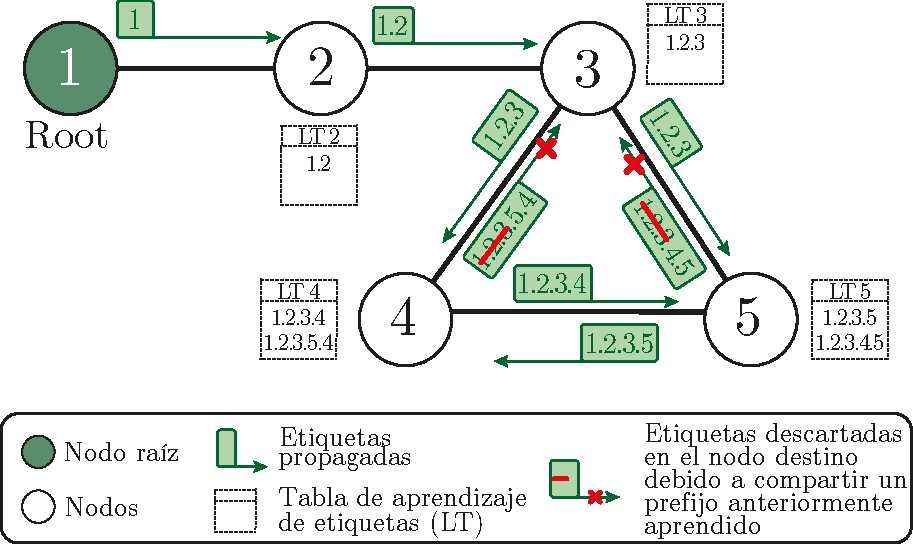
\includegraphics[width=0.6\linewidth]{fig/06_fault_sg/fault_sg_07.pdf}
    \caption{Funcionamiento de la primera fase del algoritmo DEN2NE.}
    \label{fig:labelspropagation}
\end{figure}


Una vez finalizado el proceso de etiquetado en toda la red, se considera completa la primera fase del algoritmo. La segunda fase de \gls{d2e} consiste en seleccionar la mejor etiqueta por nodo para la redistribución de carga, basándose en los criterios definidos en el propio algoritmo (Ver Sección~\ref{subsec:fase2}). En este ejemplo, los nodos con una sola etiqueta no necesitan aplicar esta fase. Sin embargo, los nodos 4 y 5 deberán elegir qué etiqueta utilizarán, ya que esta determinará posteriormente cómo redistribuirán la carga dentro de la \gls{sg}. La tercera fase del algoritmo se centra en la redistribución de cargas entre los nodos (Ver Sección~\ref{subsec:fase3}). Esta fase parte de la suposición de que todos los nodos han seleccionado una etiqueta, es decir, una ruta para llegar al nodo raíz. Como resultado, se formará una topología lógica sobre la topología física de la \gls{sg}, lo que puede dejar ciertos enlaces sin utilizar. Esto permite una distribución óptima de la energía dentro de la \gls{sg}, como se ilustra en la Figura~\ref{fig:load_power_balancing} (b). En resumen, \gls{d2e} primero explora toda la topología de la red (asignando etiquetas durante el proceso), luego define el orden a seguir para la distribución de recursos (este orden está representado por la etiqueta seleccionada) y, finalmente, reconfigura la red en función de dicho orden.\\
\\
En este trabajo, se evalúan varios modelos de \gls{ml} y \gls{dl} para apoyar al algoritmo \gls{d2e} durante su segunda fase. Más concretamente, estos modelos proporcionarán información adicional para mejorar la selección de etiquetas (y, por ende, el orden de distribución de recursos), ya que serán elegidas considerando la predicción de posibles fallos que puedan surgir en la \gls{sg}, lo que, en última instancia, mejorará el proceso de reconfiguración en su conjunto. Es importante destacar que, aunque evaluamos estos modelos exclusivamente con \gls{d2e}, tanto nuestro conjunto de datos como nuestro análisis de técnicas de IA también podrían servir como base para analizar otros algoritmos de reconfiguración en redes \gls{sg}. En definitiva, las técnicas examinadas en nuestro estudio ofrecen información complementaria sobre la predicción de fallos, y queda a discreción del mecanismo de reconfiguración específico incorporar dicha información para mejorar su procedimiento.

\section{Evaluación}

Considerando el objetivo de este trabajo, que busca detectar y predecir errores, o fallos más específicamente, es necesario definir primero un criterio de error para etiquetar los resultados del algoritmo. Dado que las simulaciones están configuradas con un escenario real que contempla pérdidas y limitaciones de capacidad en los enlaces, se decide establecer la condición de fallo en función de la presencia de un exceso de capacidad en un intercambio de energía entre dos nodos de la red. Estos errores no se introducen de forma arbitraria, sino que se simula el balance de potencia en base a la configuración establecida de la \gls{sg}. En los escenarios donde ocurren pérdidas por exceso de capacidad, se indica que, para una entrada determinada del dataset, bajo esas condiciones específicas, se producirá un fallo en la red. Posteriormente, nuestro objetivo es clasificar si ocurrirá un fallo en función de condiciones y configuraciones predefinidas. En este paso, se decide aplicar una configuración de enlaces basada en el \gls{ieee} 123 Node Test Feeder~\cite{Schneider17} para garantizar que el proceso de asignación de capacidades a los enlaces sea realista. Para simplificar, en la Tabla~\ref{tab:links} se definen tres tipos de enlaces.


\begin{table}[h!]
    \centering
    \begin{tabular}{|c|c|c|}
    \hline
    \multicolumn{1}{|c|}{\textit{R (ohm/km)}} & \multicolumn{1}{c|}{\textit{I max (A)}} & \textit{Sección (mm²)} \\ \hline
    0.272 & 185 & 70 \\ \hline
    0.78 & 100 & 25 \\ \hline
    1.91 & 53 & 10 \\ \hline
    \end{tabular}
    \caption{Configuración de enlaces basada en la topología IEEE 123 Node Test Feeder.}
    \label{tab:links}
\end{table}

Una vez que la definición de error está clara, en esta sección se evaluarán diversas técnicas de \gls{ml} y \gls{dl} en términos de predicción de error. En particular, se definen \gls{rf} y \gls{svm} como métodos de \gls{ml}, y \gls{ann} como un método de \gls{dl}, en función de sus características estructurales. Nuestra evaluación sigue el flujo de trabajo ilustrado en la Figura~\ref{fig:fault_sg_08}, en el cual, primero se genera un conjunto exhaustivo de topologías aleatorias haciendo uso de \gls{brite}, y luego se les añaden características reales, como consumo y generación por nodo, condiciones climáticas (empleando el dataset final \textit{KeyMonData}). El siguiente paso es la configuración del entorno de simulación utilizando \gls{d2e}, y finalmente se realiza un análisis detallado de los distintos modelos de \gls{ml} y \gls{dl}, cada uno de los cuales, una vez entrenados, serán capaces de predecir si una ruta obtenida por \gls{d2e} dará lugar a un error, exponiendo la capacidad de reconfigurar de forma proactiva la red.


\begin{figure}[H]
  \centering
  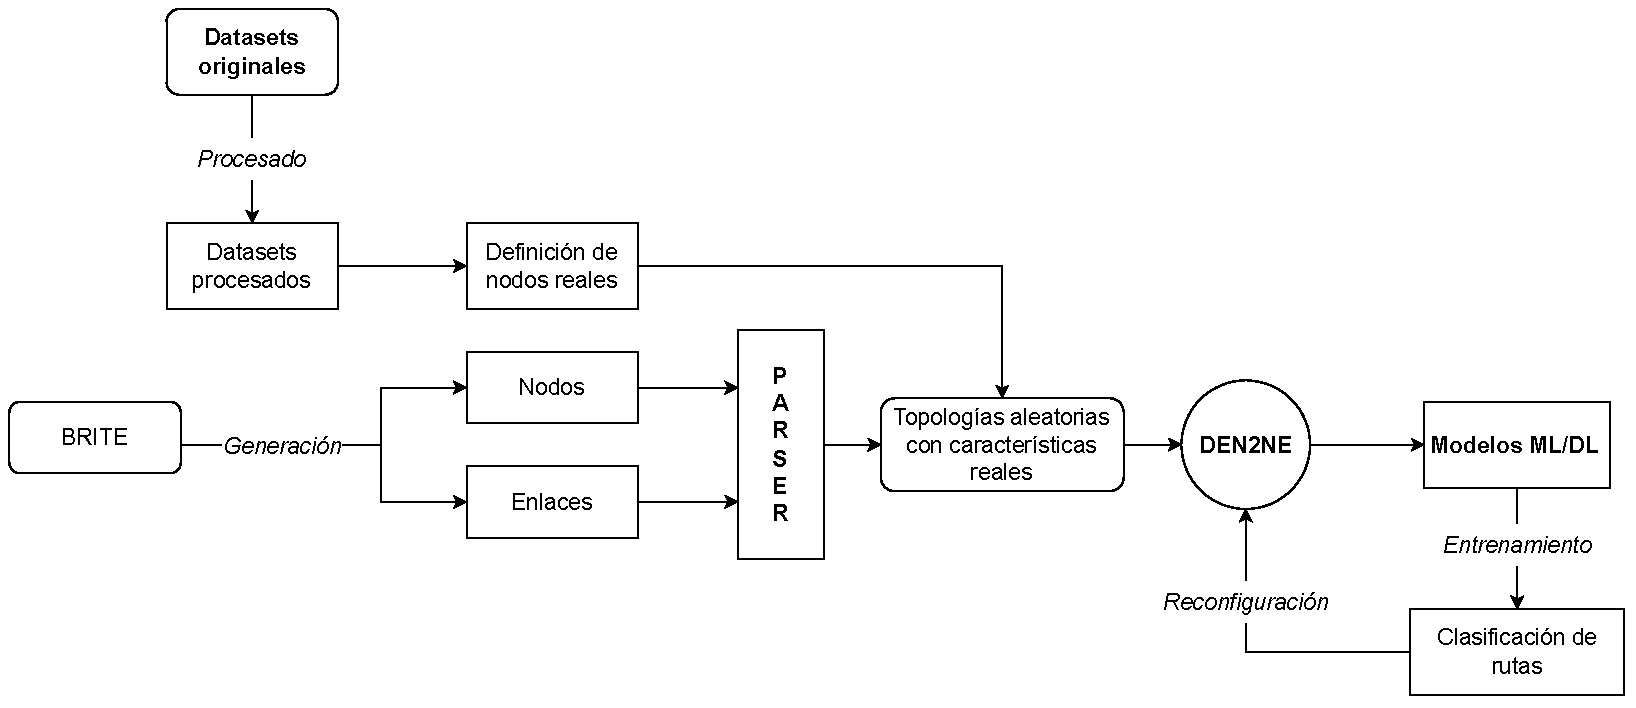
\includegraphics[width=\textwidth]{fig/06_fault_sg/fault_sg_08.drawio.pdf}
  \caption{Definición de la \textit{pipeline} para detectar y predecir errores durante el proceso de distribución de energía.}
  \label{fig:fault_sg_08}
\end{figure}


El proceso de generación aleatoria de topologías desempeña un papel fundamental en la validación y prueba de los modelos de \gls{ml} y \gls{dl}. La creación de escenarios de red diversos establece una base sólida para la detección y predicción precisa de fallos en redes \gls{sg} reales.  Para ello, de igual forma que en el Capítulo~\ref{ch:den2ne}, se empleó el generador de topologías aleatorias \gls{brite}. Un aspecto clave de este trabajo es la automatización de la generación de topologías, ya que resulta esencial para llevar a cabo simulaciones a gran escala y posibilitar una evaluación exhaustiva de los modelos de \gls{ml} y \gls{dl} en la detección de errores. Mediante el uso de scripts personalizados, se automatiza la generación de topologías con \gls{brite}, obteniendo un total de 180 topologías que posteriormente se utilizan en diferentes ejecuciones de simulación dentro de \gls{d2e}. El número total de topologías generadas se determina como el producto de varios parámetros configurados:  

\begin{itemize}
    \item \textbf{Modelos de topología}: dos modelos, Router Waxman y Router Barabasi-Albert.  
    
    \item \textbf{Número de nodos}: se generan topologías con 100, 150 y 200 nodos.  
    
    \item \textbf{Niveles de conectividad}: se especifican tres grados distintos de conectividad, considerando que cada topología presenta un grado de 2m (debido a los enlaces bidireccionales). 
    
    \item \textbf{Semillas aleatorias}: se aplican 10 archivos de semillas diferentes para garantizar la diversidad en las topologías generadas.  
\end{itemize}  

Una vez generadas, las topologías se importan al marco de trabajo \gls{d2e}, donde el algoritmo ejecuta simulaciones para modelar la distribución de energía entre los nodos. Dichas simulaciones incorporan perfiles de carga reales previamente extraídos y procesados en la Sección~\ref{subsec:keymondata}, lo que permite reproducir procesos de distribución de energía en entornos realistas de \gls{sg}. Dado que el objetivo es detectar transacciones energéticas entre nodos que superen la capacidad de sus enlaces, se define un escenario de enlaces limitados con pérdidas. Además, en el caso de \gls{brite}, se aplican 5 archivos de semillas distintos a \gls{d2e}, lo que permite obtener simulaciones diferentes a partir de la misma topología de entrada. \\ 
\\
Considerando los parámetros configurados y las 8760 filas de datos reales disponibles (correspondientes a un año de mediciones horarias), el algoritmo podría ejecutar potencialmente hasta 47,304,000 simulaciones únicas. Sin embargo, dado que resulta ineficiente e impracticable ejecutar todas ellas, es necesario seleccionar cuidadosamente qué pruebas realizar en \gls{d2e}. En este trabajo se han elegido 12 instantes específicos de tiempo, cada uno representando una hora concreta en un día de cada mes. Para simplificar el proceso, y dado que el periodo de datos comienza el 28 de noviembre de 2010, se selecciona el día 28 de cada mes. La hora escogida para la extracción de perfiles de carga es las 11:00 de la mañana, ya que en ese intervalo suele registrarse la mayor producción promedio de energía. Esta estrategia de selección aumenta la probabilidad de encontrar intercambios energéticos que excedan la capacidad de los enlaces, generando un mayor número de fallos en el proceso de distribución. Dicho enfoque resulta crucial para entrenar de manera efectiva los modelos de \gls{ml} y \gls{dl}.

\subsection{Técnicas de Machine Learning}
\label{sec:ml}

Para detectar y predecir fallos en el proceso de distribución energética se realiza una clasificación binaria de las instancias del conjunto de datos empleando dos técnicas supervisadas de \gls{ml}: \gls{rf} y \gls{svm}. El \gls{rf}  combina múltiples árboles de decisión y obtiene la predicción final por votación mayoritaria; cada árbol divide el espacio de características siguiendo criterios como la entropía o el índice de Gini, lo que le aporta robustez frente al ruido y capacidad de modelar interacciones no lineales entre variables. Por su parte, el \gls{svm} (Support Vector Machine) busca el hiperplano óptimo que maximice la separación entre las dos clases; su comportamiento frente a no linealidades se ajusta mediante el tipo de kernel y el parámetro \(\gamma\), mientras que el parámetro de regularización \(C\) controla el equilibrio entre margen y errores de clasificación.\\
\\
El desarrollo práctico de ambos modelos sigue una secuencia de pasos estándar para garantizar modelos bien entrenados y comparables: limpieza y normalización de los datos (especialmente relevante para \gls{svm}), selección/ingeniería de características, particionado en conjuntos de entrenamiento y evaluación (p. ej. \textit{train/validation/test}), tratamiento de desequilibrios de clase (p. ej. ponderación de clases o técnicas como SMOTE), búsqueda de hiperparámetros mediante \textit{grid} o \textit{random search} y validación cruzada estratificada para estimar rendimiento. Finalmente, la implementación y experimentación se realiza con la biblioteca \textit{scikit-learn}, aprovechando sus utilidades para ajuste de modelos, validación cruzada y métricas, lo que facilita la reproducibilidad y comparación sistemática entre las configuraciones.

\subsubsection{Puntuación de características}
\label{sec:puntua}

En este primer paso se diseña un modelo por defecto para cada técnica de \gls{ml}, con el fin de identificar qué características del conjunto de datos resultan más relevantes en el proceso de clasificación. Para la técnica de \gls{rf}, se entrena un modelo utilizando 10 estimadores y el criterio de entropía. La importancia de las características del conjunto de datos se estima a través del método \textit{feature\_importances\_} proporcionado por el clasificador. Este cálculo se basa en la media y la desviación estándar de la reducción de impureza que ocurre en cada árbol. En la Figura~\ref{fig:fault_sg_09} se muestran los valores relativos de importancia asignados a cada característica, cuya suma total es igual a 1. Se observa un impacto significativo en la distancia entre nodos y en los parámetros derivados de \gls{d2e} (\textit{total\_balance} y \textit{abs\_flux}), que corresponden respectivamente a la carga del nodo root tras el balanceo energético y al flujo total de recursos intercambiados en el proceso de distribución. No obstante, este método introduce un sesgo hacia aquellas características con alta cardinalidad, es decir, con un gran número de valores únicos. Dicho sesgo se debe a que estas características generan nodos de división más profundos en los árboles, al existir más opciones para particionar el conjunto de datos; por ello, tienen mayor probabilidad de recibir puntuaciones más altas de importancia. Teniendo esto en cuenta, se emplea el método de importancia por permutación como análisis comparativo. En este segundo método, los valores de cada característica se permutan aleatoriamente de manera individual, evaluando el rendimiento del clasificador en cada iteración. Así, una característica que provoca una disminución significativa en la precisión del modelo al ser permutada recibe una puntuación más alta en importancia. En este caso, como se muestra en la Figura~\ref{fig:fault_sg_10}, los parámetros derivados de \gls{d2e} (\textit{total\_balance} y \textit{abs\_flux}) mantienen puntuaciones elevadas de importancia; sin embargo, ahora también la longitud de las etiquetas de los nodos y la capacidad de los enlaces presentan una relevancia destacada.\\
\\
Para la técnica de \gls{svm}, se entrena un modelo por defecto con un kernel de Función de Base Radial (RBF), adecuado para conjuntos de datos no linealmente separables. En consecuencia, la importancia de las características del conjunto de datos se evalúa a través de los métodos \textit{support\_vectors\_} y \textit{dual\_coef\_} proporcionados por la clase. Tal como se ilustra en la Figura~\ref{fig:fault_sg_10}, los resultados indican que la longitud de las etiquetas de origen y destino ejerce una influencia significativa en el conjunto de datos. De manera análoga a lo realizado con \gls{rf}, se aplica el método de permutación, obteniéndose resultados similares. Se observa que la longitud de las etiquetas, la capacidad de los enlaces y el flujo energético total (\textit{abs\_flux}) se destacan en la clasificación.

\begin{figure}[H]
  \centering
  \includegraphics[width=\textwidth]{fig/06_fault_sg/fault_sg_09.png}
  \caption{Puntuación de la importancia de las características para el RF utilizando el método \textit{feature\_importances\_}.}
  \label{fig:fault_sg_09}
\end{figure}

\begin{figure}[H]
  \centering
  \includegraphics[width=\textwidth]{fig/06_fault_sg/fault_sg_10.png}
  \caption{Puntuación de la importancia de las características para el RF utilizando el método \textit{permutation\_importance}.}
  \label{fig:fault_sg_10}
\end{figure}

\begin{figure}[H]
  \centering
  \includegraphics[width=\textwidth]{fig/06_fault_sg/fault_sg_11.png}
  \caption{Puntuación de importancia de las características para el SVM utilizando los métodos \textit{support\_vectors\_} y  \textit{dual\_coef\_}.}
  \label{fig:fault_sg_11}
\end{figure}


\subsubsection{Optimización de hiperparámetros}

Para encontrar la mejor combinación de hiperparámetros en cada modelo se emplea el método \textit{Grid Search}. Este método realiza una búsqueda exhaustiva dentro de una cuadrícula de hiperparámetros con el fin de identificar la combinación que ofrece la mayor precisión del modelo.\\
\\
En el caso de la técnica \gls{rf}, el análisis se centró en dos hiperparámetros principales: el número de estimadores o árboles y el criterio de medida de impureza (basado en la entropía o en Gini). La ejecución del método determinó, a partir de los métodos \textit{best\_score\_} y \textit{best\_params\_}, la mejor combinación de hiperparámetros, alcanzando una precisión del 99.18\% con un clasificador de 100 estimadores empleando el criterio de entropía (Tabla~\ref{tab:rfgs_precision}). Para un análisis más detallado, se utilizó el atributo \textit{cv\_results\_}, que proporcionó información completa sobre la búsqueda. Se observa que, aunque las variaciones en la precisión entre las distintas combinaciones de parámetros fueron mínimas, los tiempos de ajuste mostraron diferencias significativas. Tal como se presenta en la Tabla~\ref{tab:rfgs_tiempo}, la duración del entrenamiento aumentó de forma proporcional al número de estimadores configurados en el modelo. Por lo tanto, dado que la precisión no mejoró de manera significativa al superar los 25 estimadores, se determinó que el clasificador con 25 estimadores y criterio de entropía constituye el modelo más óptimo.

% Primera tabla: Precisión
\begin{table}[H]
\centering
\begin{tabular}{|c|c|c|}
\hline
\multirow{2}{*}{\textbf{Número de estimadores}} & \multicolumn{2}{c|}{\textbf{Criterio}} \\ \cline{2-3}
 & \textit{\textbf{Entropía}} & \textit{\textbf{Gini}} \\ \hline
10  & 99.07 & 99.02 \\ \hline
25  & 99.16 & 99.14 \\ \hline
50  & 99.16 & 99.15 \\ \hline
75  & 99.17 & 99.17 \\ \hline
100 & 99.18 & 99.16 \\ \hline
\end{tabular}
\caption{Evolución de la Precisión (\%) aplicando la búsqueda (\textit{Grid Search}) sobre el RF.}
\label{tab:rfgs_precision}
\end{table}

% Segunda tabla: Tiempo
\begin{table}[H]
\centering
\begin{tabular}{|c|c|c|}
\hline
\multirow{2}{*}{\textbf{Número de estimadores}} & \multicolumn{2}{c|}{\textbf{Criterio}} \\ \cline{2-3}
 & \textit{\textbf{Entropía}} & \textit{\textbf{Gini}} \\ \hline
10   & 147  & 146  \\ \hline
25   & 373  & 382  \\ \hline
50   & 747  & 761  \\ \hline
75   & 1072 & 1002 \\ \hline
100  & 1439 & 987  \\ \hline
\end{tabular}
\caption{Evolución del Tiempo (s) de entrenamiento del RF en función del número de estimadores.}
\label{tab:rfgs_tiempo}
\end{table}


Para modelar una \gls{svm} óptima se estudiaron principalmente dos hiperparámetros: el tipo de núcleo (\textit{kernel}) y el parámetro de regularización \textit{C} (véase Tablas~\ref{tab:svmgs} y \ref{tab:svmgs2}). El parámetro \( \gamma \) fue omitido debido al escalado previo de los datos, que eliminó su influencia. En este caso, a diferencia de la técnica \gls{rf}, la búsqueda de la mejor combinación de hiperparámetros requirió un mayor tiempo de ejecución, alcanzando aproximadamente las 350 horas.  Los resultados de este proceso mostraron que el modelo óptimo correspondía a una \gls{svm} con núcleo RBF y un parámetro de regularización \textit{C} igual a 1, logrando una precisión del 97.78\% y requiriendo, además, un tiempo de entrenamiento relativamente bajo en comparación con otras combinaciones de hiperparámetros.  

%TABLA 4.4
\begin{table}[H]
  \centering
  \caption{Resultados extraídos del método \textit{cv\_results\_} de la búsqueda \textit{Grid Search} en la SVM.}
  \begin{subtable}{0.45\linewidth}
    \centering
    \caption{Precisión (\%) (\textit{mean\_test\_score})}
    \begin{tabular}{|>{}c |c|c|c|}
      \hline
      \textit{\begin{tabular}[c]{@{}c@{}}\textbf{Kernel} /\\\textbf{C}\end{tabular}} & \textit{poly} & \textit{rbf} & \textit{sigmoid}\\ \hline
      0.25 & 97.65 & 97.66 & 95.96 \\ \hline
      0.5 & 97.65 & 97.71 & 95.94 \\ \hline
      0.75 & 97.65 & 97.75 & 95.82 \\ \hline
      1 & 97.65 & 97.78 & 95.81 \\ \hline
    \end{tabular}
    \label{tab:svmgs}
  \end{subtable}
  \hfill
  \begin{subtable}{0.45\linewidth}
    \centering
    \caption{Tiempo (s) (\textit{mean\_fit\_time})}
    \begin{tabular}{|>{}c |c|c|c|}
      \hline
      \textit{\begin{tabular}[c]{@{}c@{}}\textbf{Kernel} /\\\textbf{C}\end{tabular}} & \textit{poly} & \textit{rbf} & \textit{sigmoid}\\ \hline
      0.25 & 21030 & 13876 & 14659 \\ \hline
      0.5 & 28807 & 10277 & 18695 \\ \hline
      0.75 & 42183 & 9328 & 12235 \\ \hline
      1 & 47460 & 9446 & 12869 \\ \hline
    \end{tabular}
    \label{tab:svmgs2}
  \end{subtable}
  \label{tab:svmgs_combined}
\end{table}

El análisis del atributo \textit{cv\_results\_} reveló que el núcleo \textit{sigmoid} ofreció el peor desempeño, mientras que el núcleo polinómico (\textit{poly}) presentó un aumento del tiempo de entrenamiento a medida que se incrementaba el valor de \textit{C}, lo que sugiere que un valor elevado de este parámetro no resulta adecuado para dicho núcleo.  

\subsubsection{Reducción de dimensionalidad}

Tras analizar las mejores combinaciones de hiperparámetros para cada técnica de \gls{ml}, se estudia la aplicación de algunas metodologías de reducción de dimensionalidad sobre el dataset. El objetivo es eliminar información irrelevante o redundante para lograr un entrenamiento de modelos más eficiente. Se probaron dos técnicas diferentes con el fin de comparar posteriormente el rendimiento de los modelos \gls{rf} y \gls{svm} en la sección de resultados. \\
\\
El primero de ellos es \gls{rfecv}. Este método descarta de manera iterativa las características menos influyentes hasta que el rendimiento del modelo deja de mejorar significativamente. Con una validación cruzada de 5-\textit{folds}, puede observarse en la Figura~\ref{fig:fault_sg_12} que la máxima precisión para el modelo óptimo de \gls{rf} se alcanzó con ocho características. Además, se confirmó que las características identificadas (\textit{cap}, \textit{dist}, \textit{origen\_id}, \textit{dest\_id}, \textit{len\_origen\_tag}, \textit{len\_dest\_tag}, \textit{total\_balance}, \textit{abs\_flux}) coincidían con aquellas que obtuvieron las puntuaciones más altas en la Sección~\ref{sec:puntua}. Sin embargo, en el caso de \gls{svm}, la clase del clasificador no contaba con los atributos necesarios para implementar \gls{rfecv} (\textit{coef\_}, \textit{feature\_importances\_}), por lo que esta técnica solo se aplicó a \gls{rf}.  
    
\begin{figure}[H]
\centering
\includegraphics[width=0.65\textwidth]{fig/06_fault_sg/fault_sg_12.png}
\caption{Análisis de la precisión del modelo RF basado en el número de características utilizadas con el método RFECV.}
\label{fig:fault_sg_12}
\end{figure}
    
El segundo método que se implementó fue \gls{pca}, el cual, reduce la dimensionalidad del conjunto de datos utilizando la técnica \gls{svd}. Su funcionamiento se basa en encontrar las direcciones principales de variación (\textit{k} vectores) en el conjunto de datos para construir una matriz de proyección, que establece un nuevo espacio de características de dimensión \textit{k}. Para definir el número óptimo de componentes, se empleó el método del codo. La Figura~\ref{fig:fault_sg_13} muestra que la varianza se estabiliza en tres componentes, por lo que, con fines comparativos, se estudió el rendimiento de \gls{rf} y \gls{svm} para dos y cuatro componentes.  El tercer método es la selección de características univariada, el cual, utiliza el método \textit{SelectKBest()} que requiere un escalado previo y la especificación de un número fijo de características con las que trabajar. En este caso, se seleccionaron valores de \textit{k} iguales a cinco y ocho características.  
    

\begin{figure}[H]
\centering
\includegraphics[width=0.65\textwidth]{fig/06_fault_sg/fault_sg_13.png}
\caption{Análisis de varianza basado en el número de componentes utilizados en el PCA.}
\label{fig:fault_sg_13}
\end{figure}

\subsection{Técnicas de Deep Learning}
\label{sec:dl}

El desarrollo de las técnicas de \gls{dl} se dividió en el diseño óptimo y el entrenamiento de dos modelos de \gls{ann}, empleando dos bibliotecas diferentes: \textit{Scikit-Learn} y el módulo \textit{Keras} de \textit{TensorFlow}. Las \glspl{ann}, y en particular las \glspl{mlp}, se componen de múltiples capas de nodos y conexiones que imitan la estructura neuronal del cerebro humano. En cuanto a su desarrollo, cabe destacar que se omitieron las etapas de puntuación de características y de reducción de dimensionalidad aplicadas a los modelos de \gls{ml} en la Sección~\ref{sec:ml}. Esto se debe a que las \glspl{ann} son capaces de analizar internamente y ponderar la relevancia de las características dentro de la red, por lo que dichos pasos no resultan necesarios en este caso.  

\subsubsection{Optimización de hiperparámetros}

En esta etapa se lleva a cabo el ajuste de hiperparámetros con el fin de lograr un rendimiento óptimo de una \gls{ann}. Para ello, se aplica el método Grid Search al modelo \gls{mlp} proporcionado por la biblioteca \textit{Scikit-Learn}. El estudio se centra en la configuración de las capas ocultas y el número de neuronas por capa (\textit{hidden\_layer\_sizes}), así como en otros hiperparámetros como la función de activación (\textit{activation}) y el algoritmo de optimización (\textit{solver}). Para evitar el sobreajuste durante la ejecución de Grid Search, se establece un máximo de 100 iteraciones junto con la técnica de \textit{early stopping}, que se activa si no se producen mejoras significativas en 10 iteraciones consecutivas. 

Se ha estimado que el proceso completo de búsqueda requiere aproximadamente 2.34 horas en un servidor con 32 procesadores. En la Tabla~\ref{tab:mlpaccuracy} se observa que el algoritmo de optimización Stochastic Gradient Descent supera, en general, al algoritmo \textit{Adam}. En cuanto a los tiempos de entrenamiento, la Tabla~\ref{tab:mlptiempo} refleja el impacto tanto de la estructura de capas como del número de neuronas configuradas en la red. De manera similar, las dimensiones también influyen en las precisiones alcanzadas, registrándose algunos casos de sobreajuste que derivaron en menores tasas de clasificación.  


\begin{table}[H]
    \centering
    \begin{tabular}{|
    >{}c |cc|cc|}
    \hline
    \textit{\textbf{Solver}} & \multicolumn{2}{c|}{\textit{adam}} & \multicolumn{2}{c|}{\textit{sgd}} \\ \hline
    \textit{\begin{tabular}[c]{@{}c@{}}\textbf{Función de activación} /\\ \textbf{Capas ocultas}\end{tabular}} & \multicolumn{1}{c|}{\textit{relu}} & \textit{tanh} & \multicolumn{1}{c|}{\textit{relu}} & \textit{tanh} \\ \hline
    (5,) & \multicolumn{1}{c|}{90.17} & \multicolumn{1}{c|}{97.61} & \multicolumn{1}{c|}{97.66} & \multicolumn{1}{c|}{97.54} \\ \hline
    (8,) & \multicolumn{1}{c|}{92.03} & \multicolumn{1}{c|}{89.73} & \multicolumn{1}{c|}{97.65} & \multicolumn{1}{c|}{97.65} \\ \hline
    (10,) & \multicolumn{1}{c|}{87.00} & \multicolumn{1}{c|}{89.90} & \multicolumn{1}{c|}{97.48} & \multicolumn{1}{c|}{89.76} \\ \hline
    (50,) & \multicolumn{1}{c|}{86.89} & \multicolumn{1}{c|}{89.82} & \multicolumn{1}{c|}{89.53} & \multicolumn{1}{c|}{97.65} \\ \hline
    (100,) & \multicolumn{1}{c|}{90.95} & \multicolumn{1}{c|}{89.71} & \multicolumn{1}{c|}{84.56} & \multicolumn{1}{c|}{89.72} \\ \hline
    (5, 5) & \multicolumn{1}{c|}{89.80} & \multicolumn{1}{c|}{89.72} & \multicolumn{1}{c|}{97.66} & \multicolumn{1}{c|}{97.65} \\ \hline
    (8, 8) & \multicolumn{1}{c|}{88.49} & \multicolumn{1}{c|}{89.72} & \multicolumn{1}{c|}{89.89} & \multicolumn{1}{c|}{97.65} \\ \hline
    (10, 10) & \multicolumn{1}{c|}{81.68} & \multicolumn{1}{c|}{89.70} & \multicolumn{1}{c|}{90.30} & \multicolumn{1}{c|}{97.65} \\ \hline
    (50, 50) & \multicolumn{1}{c|}{81.91} & \multicolumn{1}{c|}{82.04} & \multicolumn{1}{c|}{97.66} & \multicolumn{1}{c|}{89.73} \\ \hline
    \end{tabular}
    \caption{Precisión (\%) (\textit{mean\_test\_score}) extraída del método \textit{cv\_results\_} del MLP.}
    \label{tab:mlpaccuracy}
\end{table}

\begin{table}[H]
    \centering
    \begin{tabular}{|
    >{}c |cc|cc|}
    \hline
    \textit{\textbf{Solver}} & \multicolumn{2}{c|}{\textit{adam}} & \multicolumn{2}{c|}{\textit{sgd}} \\ \hline
    \textit{\begin{tabular}[c]{@{}c@{}}\textbf{Función de activación} /\\ \textbf{Capas ocultas}\end{tabular}} & \multicolumn{1}{c|}{\textit{relu}} & \textit{tanh} & \multicolumn{1}{c|}{\textit{relu}} & \textit{tanh} \\ \hline
    (5,) & \multicolumn{1}{c|}{88} & \multicolumn{1}{c|}{37} & \multicolumn{1}{c|}{63} & \multicolumn{1}{c|}{35} \\ \hline
    (8,) & \multicolumn{1}{c|}{96} & \multicolumn{1}{c|}{43} & \multicolumn{1}{c|}{35} & \multicolumn{1}{c|}{36} \\ \hline
    (10,) & \multicolumn{1}{c|}{94} & \multicolumn{1}{c|}{40} & \multicolumn{1}{c|}{56} & \multicolumn{1}{c|}{43} \\ \hline
    (50,) & \multicolumn{1}{c|}{157} & \multicolumn{1}{c|}{168} & \multicolumn{1}{c|}{143} & \multicolumn{1}{c|}{70} \\ \hline
    (100,) & \multicolumn{1}{c|}{236} & \multicolumn{1}{c|}{223} & \multicolumn{1}{c|}{170} & \multicolumn{1}{c|}{131} \\ \hline
    (5, 5) & \multicolumn{1}{c|}{136} & \multicolumn{1}{c|}{50} & \multicolumn{1}{c|}{52} & \multicolumn{1}{c|}{44} \\ \hline
    (8, 8) & \multicolumn{1}{c|}{159} & \multicolumn{1}{c|}{54} & \multicolumn{1}{c|}{69} & \multicolumn{1}{c|}{46} \\ \hline
    (10, 10) & \multicolumn{1}{c|}{149} & \multicolumn{1}{c|}{55} & \multicolumn{1}{c|}{54} & \multicolumn{1}{c|}{48} \\ \hline
    (50, 50) & \multicolumn{1}{c|}{333} & \multicolumn{1}{c|}{319} & \multicolumn{1}{c|}{166} & \multicolumn{1}{c|}{155} \\ \hline
    \end{tabular}
    \caption{Tiempo (s) (\textit{mean\_fit\_time}) extraída del método \textit{cv\_results\_} del MLP.}
    \label{tab:mlptiempo}
\end{table}

Por tanto, el análisis de resultados determina que la configuración óptima del \gls{mlp} está formada por dos capas ocultas de 5 neuronas cada una (estructura (5,5)), función de activación \gls{relu} y algoritmo de optimización SGD (solver). Las Figuras~\ref{fig:fault_sg_14} y \ref{fig:fault_sg_15} muestran, respectivamente, la evolución de la precisión y de la función de pérdidas durante el entrenamiento. El modelo óptimo converge en la iteración (\textit{epoch}) 41, alcanzando una precisión del 97.66\% y un valor de la función de pérdida de 0.0712.


\begin{figure}[H]
  \centering
  \includegraphics[width=0.85\textwidth]{fig/06_fault_sg/fault_sg_14.png}
  \caption{Evolución de la precisión del ANN de \textit{Scikit-Learn}.}
  \label{fig:fault_sg_14}
\end{figure}

\begin{figure}[H]
  \centering
  \includegraphics[width=0.85\textwidth]{fig/06_fault_sg/fault_sg_15.png}
  \caption{Evolución de la función de pérdidas para la ANN de S\textit{cikit-Learn}.}
  \label{fig:fault_sg_15}
\end{figure}

Tras identificar la configuración de hiperparámetros óptima para el \gls{mlp} mediante \textit{Grid Search} sobre la implementación de \textit{Scikit-Learn}, dicha configuración se replicó en un modelo \gls{ann} equivalente implementado con el módulo \textit{Keras} de \textit{TensorFlow}. El objetivo de esta réplica es comprobar la consistencia de los resultados y verificar que dos implementaciones distintas de redes neuronales con la misma arquitectura e hiperparámetros alcanzan comportamientos comparables en términos de convergencia, precisión y función de pérdidas.\\
\\
En las Figuras~\ref{fig:fault_sg_16} y \ref{fig:fault_sg_17} se muestra la evolución de la precisión y de la función de pérdidas durante el entrenamiento del \gls{ann} en \textit{Keras}. A diferencia del \gls{mlp} de \textit{Scikit-Learn}, que alcanzó convergencia en la iteración 41 bajo la estrategia de \textit{early stopping}, la implementación en \textit{Keras} completó las 100 iteraciones programadas; aun así, los resultados finales son muy similares: la pérdida en la última iteración es aproximadamente 0.068 y la precisión alcanzada ronda el 97.87\%. Estas cifras corroboran la reproducibilidad del diseño elegido y apuntan a una estabilidad del modelo frente a diferencias internas entre librerías (por ejemplo, implementaciones del optimizador, inicialización de pesos o manejo del \textit{early stopping}). En conjunto, los experimentos muestran que la configuración propuesta para la red neuronal es robusta y proporciona un rendimiento elevado y consistente para la tarea de predicción de fallos en reconfiguración de \glspl{sg}.

\begin{figure}[H]
\centering
\includegraphics[width=0.8\textwidth]{fig/06_fault_sg/fault_sg_16.png}
\caption{Evolución de la precisión para el ANN implementado en \textit{Keras}.}
\label{fig:fault_sg_16}
\end{figure}

\begin{figure}[H]
\centering
\includegraphics[width=0.8\textwidth]{fig/06_fault_sg/fault_sg_17.png}
\caption{Evolución de la función de pérdidas para el ANN implementado en \textit{Keras}.}
\label{fig:fault_sg_17}
\end{figure}



\section{Resultados y discusión de los modelos entrenados} 

Los resultados recogidos en la Tabla~\ref{tab:resumen} ofrecen una visión global del rendimiento de los modelos estudiados. Para validar los modelos de \gls{ml} se han empleado dos métodos complementarios: la matriz de confusión (y sus métricas derivadas) y la validación cruzada \emph{K-Fold}. En el caso de las técnicas de \gls{dl}, además de la matriz de confusión, se han usado las métricas que proveen \textit{Scikit-Learn} y \textit{Keras} (pérdidas y precisión) durante el entrenamiento y la validación.\\
\\
A continuación se presentan los resultados y su discusión para cada familia de modelos; primero se exponen los resultados obtenidos y, a continuación, se interpretan sus implicaciones prácticas y limitaciones. Al final se discute brevemente la generalización potencial a otras topologías y algoritmos de reconfiguración.

\subsection{Random Forest} 

La matriz de confusión proporciona métricas esenciales para evaluar el rendimiento del modelo \gls{rf}. Si nos fijamos únicamente en la \textit{Accuracy}, los resultados parecen buenos en las cinco pruebas realizadas con distintas técnicas de reducción de dimensionalidad aplicadas durante el entrenamiento del \gls{rf}. No obstante, al analizar las métricas de \textit{Precision} y \textit{Recall} surgen diferencias relevantes. Por ejemplo, la aplicación de \gls{pca} con dos componentes obtiene una \textit{Accuracy} elevada (97.55\%), pero la \textit{Precision} es muy baja (12.52\%), lo que indica que el porcentaje de errores efectivamente detectados respecto al total de errores del conjunto es extremadamente reducido (0.67\%). En consecuencia, el \textit{F1 Score} también resulta muy bajo (1.27\%), ya que combina \textit{Precision} y \textit{Recall}.\\
\\
Analizando en conjunto todas las métricas ofrecidas por la matriz de confusión, se concluye que la técnica de reducción de dimensionalidad que mejor funciona para entrenar el \gls{rf} es \gls{rfecv}. Este método presenta el menor coste en predicción de errores porque reduce tanto la probabilidad de falsas alarmas como la de no detectar errores reales, alcanzando altas tasas de \textit{Precision} (94.28\%) y \textit{Recall} (81.05\%). Como segunda mejor opción para la detección y predicción de errores se sitúa el uso de todas las características del conjunto de datos, sin aplicar reducción alguna.\\
\\
Los resultados obtenidos mediante la validación cruzada \textit{K-Fold} muestran las mismas tendencias en \textit{accuracy} que las derivadas de la matriz de confusión, lo que confirma la robustez y buena generalización del enfoque con \gls{rfecv} en nuestro conjunto de datos.

\subsection{Support Vector Machine} 

Para evaluar el rendimiento del modelo \gls{svm} conviene subrayar el elevado coste computacional y temporal requerido para su entrenamiento: en nuestro caso fueron necesarias aproximadamente 325 horas para ejecutar y validar las 5 pruebas. En la matriz de confusión se observa de inmediato que, en ambos casos en los que se aplicó \gls{pca}, aparecen valores indefinidos para las métricas de \textit{Precision} y \textit{F1 Score}; esto se debe a que el modelo \gls{svm} no realiza predicciones de la clase de interés (es decir, no predice ejemplares positivos), por lo que dichas métricas no pueden calcularse.\\
\\
Aunque el porcentaje de \textit{Accuracy} resulte alto (97.61\%), el modelo no está realizando una clasificación útil para nuestro objetivo, y el coste asociado a errores (falsos negativos/falsos positivos según el caso) es elevado. Respecto a la \textit{Precision}, los mejores resultados se obtienen al no aplicar ninguna técnica de reducción de dimensionalidad (89.32\%); en cambio, con la selección univariante de características (\textit{SelectKBest}) la eficiencia disminuye al reducir el número de características (por ejemplo, 65.25\% con menos variables). Por otra parte, la métrica \textit{Recall} presenta valores bajos en todas las pruebas, lo que indica que la proporción de fallos correctamente identificados es muy pequeña.\\
\\
Con base en este análisis se concluye que el \gls{svm} no resulta suficientemente eficiente para el objetivo de detección y predicción de fallos en nuestro contexto. La validación por \textit{K-Fold} arroja valores de \textit{accuracy} similares a los de la matriz de confusión (como ocurría con el \gls{rf}), pero las limitaciones comentadas: alto coste computacional; baja capacidad para identificar la clase positiva; y sensibilidad a la reducción de dimensionalidad, hacen que descartemos el uso de \gls{svm} para detección de errores en \gls{sg}. Estos resultados aportan una justificación sólida para priorizar modelos alternativos más adecuados a la naturaleza del problema.


\subsection{ANNs} 

Dado que en el desarrollo de las técnicas de \gls{dl} no se aplicaron pasos dedicados de puntuación de características ni de reducción de dimensionalidad, la evaluación se centra en la comparación de los resultados obtenidos por las dos \gls{ann} desarrolladas. Como se indicó en la Sección~\ref{sec:dl}, el rendimiento de ambos \gls{ann} es muy similar: las precisiones alcanzadas son prácticamente idénticas (97.84\%) y las demás métricas derivadas de la matriz de confusión muestran diferencias mínimas entre ambos modelos. Se observa un \textit{Recall} ligeramente superior en la \gls{ann} de \textit{Scikit-Learn} (14.98\%), si bien ambos modelos evidencian una eficacia reducida en la detección de fallos reales. Por su parte, la \gls{ann} implementada con \textit{Keras} presenta una \textit{Precision} mayor (72.17\%), lo que se traduce en una menor probabilidad de falsas alarmas. Además, se aplicaron los métodos de evaluación provistos por \textit{Scikit-Learn} (\texttt{score()}) y por \textit{Keras} (\texttt{evaluate()}) a ambos modelos: \texttt{score()} devuelve la precisión, mientras que \texttt{evaluate()} aporta también el valor de la función de pérdida. Los resultados siguen siendo comparables entre ambas implementaciones y, si se prioriza la detección de errores reales (\textit{recall}), la \gls{ann} de \textit{Keras} resulta la opción preferible por su menor tasa de falsas alarmas relativa.\\
\\
Por último, cabe destacar que algunos métodos \gls{ml} más sencillos (por ejemplo, \gls{rf} con \gls{rfecv}) alcanzan un \textit{Recall} mayor que las \gls{ann} aquí evaluadas. Este comportamiento puede deberse, en parte, a la eficacia de las técnicas de reducción de dimensionalidad aplicadas en los modelos \gls{ml} y a la forma distinta en que las \gls{ann} realizan internamente la ponderación y selección de características.

\begin{sidewaystable}
    %\centering
    \caption{Resumen de los resultados obtenidos del desarrollo de modelos ML y DL.}
    \resizebox{\textwidth}{!}{
    \begin{tabular}{
    >{}c 
    >{}c |llll|ll|}
    \cline{3-8}
    \multicolumn{2}{c|}{\textit{}} & \multicolumn{4}{c|}{\textbf{Matriz de confusión}} & \multicolumn{2}{c|}{\begin{tabular}[c]{@{}c@{}}\textbf{K-Fold Validación cruzada}\end{tabular}} \\ \cline{3-8} 
    \multicolumn{2}{c|}{\cellcolor[HTML]{FFFFFF}\textit{}} & \multicolumn{1}{c|}{\textit{Accuracy}} & \multicolumn{1}{c|}{\textit{Precision}} & \multicolumn{1}{c|}{\textit{Recall}} & \multicolumn{1}{c|}{\textit{F1 Score}} & \multicolumn{1}{c|}{\textit{Accuracy}} & \multicolumn{1}{c|}{\textit{Standard Deviation / Loss}} \\ \hline
    \multicolumn{1}{|c|}{} & \textit{Por defecto} & \multicolumn{1}{c|}{99.29} & \multicolumn{1}{c|}{94.40} & \multicolumn{1}{c|}{74.27} & \multicolumn{1}{c|}{83.16} & \multicolumn{1}{c|}{99.30} & \multicolumn{1}{c|}{0.02} \\ \cline{2-8} 
    \multicolumn{1}{|c|}{} & \textit{RFECV} & \multicolumn{1}{c|}{99.44} & \multicolumn{1}{c|}{94.28} & \multicolumn{1}{c|}{81.05} & \multicolumn{1}{c|}{87.17} & \multicolumn{1}{c|}{99.47} & \multicolumn{1}{c|}{0.02} \\ \cline{2-8} 
    \multicolumn{1}{|c|}{} & \textit{kbest (n=5)} & \multicolumn{1}{c|}{97.79} & \multicolumn{1}{c|}{65.97} & \multicolumn{1}{c|}{12.55} & \multicolumn{1}{c|}{21.08} & \multicolumn{1}{c|}{97.80} & \multicolumn{1}{c|}{0.02} \\ \cline{2-8} 
    \multicolumn{1}{|c|}{} & \textit{kbest (n=8)} & \multicolumn{1}{c|}{97.74} & \multicolumn{1}{c|}{53.95} & \multicolumn{1}{c|}{27.37} & \multicolumn{1}{c|}{36.32} & \multicolumn{1}{c|}{97.79} & \multicolumn{1}{c|}{0.01} \\ \cline{2-8} 
    \multicolumn{1}{|c|}{} & \textit{PCA (n=2)} & \multicolumn{1}{c|}{97.55} & \multicolumn{1}{c|}{12.52} & \multicolumn{1}{c|}{00.67} & \multicolumn{1}{c|}{01.27} & \multicolumn{1}{c|}{97.35} & \multicolumn{1}{c|}{0.01} \\ \cline{2-8} 
    \multicolumn{1}{|c|}{\multirow{-6}{*}{\begin{tabular}[c]{@{}c@{}}\textbf{Random Forest} \\ {[}25 estimadores, \\ criterio de entropía{]}\end{tabular}}} & \textit{PCA (n=4)} & \multicolumn{1}{c|}{98.06} & \multicolumn{1}{c|}{81.66} & \multicolumn{1}{c|}{22.60} & \multicolumn{1}{c|}{35.41} & \multicolumn{1}{c|}{98.04} & \multicolumn{1}{c|}{0.00} \\ \hline
    \multicolumn{1}{|c|}{} & \textit{Por defecto} & \multicolumn{1}{c|}{97.23} & \multicolumn{1}{c|}{89.32} & \multicolumn{1}{c|}{06.95} & \multicolumn{1}{c|}{12.83} & \multicolumn{1}{c|}{97.79} & \multicolumn{1}{c|}{0.01} \\ \cline{2-8} 
    \multicolumn{1}{|c|}{} & \textit{kbest (n=5)} & \multicolumn{1}{c|}{97.11} & \multicolumn{1}{c|}{65.25} & \multicolumn{1}{c|}{12.29} & \multicolumn{1}{c|}{20.73} & \multicolumn{1}{c|}{97.80} & \multicolumn{1}{c|}{0.01} \\ \cline{2-8} 
    \multicolumn{1}{|c|}{} & \textit{kbest (n=8)} & \multicolumn{1}{c|}{97.05} & \multicolumn{1}{c|}{71.19} & \multicolumn{1}{c|}{09.30} & \multicolumn{1}{c|}{16.46} & \multicolumn{1}{c|}{97.79} & \multicolumn{1}{c|}{0.01} \\ \cline{2-8} 
    \multicolumn{1}{|c|}{} & \textit{PCA (n=2)} & \multicolumn{1}{c|}{97.61} & \multicolumn{1}{c|}{-} & \multicolumn{1}{c|}{0} & \multicolumn{1}{c|}{-} & \multicolumn{1}{c|}{97.76} & \multicolumn{1}{c|}{0.00} \\ \cline{2-8} 
    \multicolumn{1}{|c|}{\multirow{-5}{*}{\begin{tabular}[c]{@{}c@{}}\textbf{SVM} \\ {[}C=1, kernel=rbf{]}\end{tabular}}} & \textit{PCA (n=4)} & \multicolumn{1}{c|}{97.61} & \multicolumn{1}{c|}{-} & \multicolumn{1}{c|}{0} & \multicolumn{1}{c|}{-} & \multicolumn{1}{c|}{97.76} & \multicolumn{1}{c|}{0.00} \\ \hline
    \multicolumn{1}{|c|}{} & \multicolumn{1}{c|}{\textit{sklearn}} & \multicolumn{1}{c|}{97.84} & \multicolumn{1}{c|}{69.03} & \multicolumn{1}{c|}{14.98} & \multicolumn{1}{c|}{24.66} & \multicolumn{1}{c|}{97.83} & \multicolumn{1}{c|}{*-} \\ \cline{2-8} 
    \multicolumn{1}{|c|}{\multirow{-2}{*}{\begin{tabular}[c]{@{}c@{}}\textbf{ANN}\\ {[}(5, 5), relu, sgd{]}\end{tabular}}} & \multicolumn{1}{c|}{\textit{keras}} & \multicolumn{1}{c|}{97.84} & \multicolumn{1}{c|}{72.17} & \multicolumn{1}{c|}{13.49} & \multicolumn{1}{c|}{22.74} & \multicolumn{1}{c|}{97.85} & \multicolumn{1}{c|}{**0.0690} \\ \hline
    \end{tabular}
    }
    
    \label{tab:resumen}
    \footnotesize{Nota: * \textit{Score()}/ ** \textit{Evaluate()}}
\end{sidewaystable}

\subsection{Generalización a otras topologías y algoritmos de reconfiguración}

Estos resultados ponen de manifiesto la eficacia de las técnicas de \gls{ml} y \gls{dl} para mejorar la fiabilidad de las \gls{sg} y ofrecen orientación práctica para el desarrollo futuro de sistemas inteligentes de gestión de red. Conviene aclarar que los modelos desarrollados no están pensados como soluciones a medida para una topología fija y concreta; por el contrario, se han optimizado empleando topologías aleatorias que varían de forma sistemática en número de nodos, grado de conectividad y modelo probabilístico (Waxman / Barabási-Albert), aplicando parámetros inspirados en el \gls{ieee} 123 Node Test Feeder para dotar de realismo y diversidad al conjunto de pruebas. Es cierto que el modelo no buscará el máximo rendimiento en una topología particular, sino que persigue un rendimiento medio óptimo sobre un amplio abanico de topologías, adoptando así una estrategia de compromiso que generaliza bien frente a condiciones de red heterogéneas.\\
\\
En coherencia con lo anterior, sería deseable en trabajos futuros estudiar de forma más profunda la adaptación de modelos específicos a topologías particulares o la comparación frente a otros algoritmos de reconfiguración (incluyendo enfoques puramente centralizados, puramente distribuidos o híbridos). Dichas investigaciones permitirían cuantificar hasta qué punto la personalización de modelos mejora el rendimiento frente a la solución generalista aquí propuesta. En cualquier caso, este estudio inicial constituye una base sólida para análisis posteriores y demuestra la capacidad de las técnicas propuestas para potenciar el algoritmo \gls{d2e}, que era el objetivo principal de esta aportación.

\section{Conclusiones}
\label{sec:conclufault}

En este trabajo hemos propuesto un enfoque novedoso para la predicción de fallos en \gls{sg} mediante la aplicación de modelos de \gls{ml} y \gls{dl} como apoyo al proceso de reconfiguración proactiva de la red. Partiendo del algoritmo \gls{d2e}, abordamos las complejidades de la redistribución de carga en \gls{sg} densas y heterogéneas aplicando técnicas avanzadas de \gls{ml}/\gls{dl} para mejorar la toma de decisiones durante la fase de reconfiguración de la red. Mediante el uso de conjuntos de datos reales como \textit{SustDataED} e integrando datos simulados de generación fotovoltaica obtenidos con herramientas como \textit{PVWatts}, este trabajo demuestra la viabilidad de emplear modelos impulsados por \gls{ai} para predecir fallos potenciales y aumentar la resiliencia del sistema.\\
\\
La metodología propuesta identificó de forma efectiva rutas óptimas para el balance de carga minimizando errores en la distribución energética. Entre los modelos evaluados, el clasificador Random Forest optimizado con \gls{rfecv} para la reducción de dimensionalidad mostró un comportamiento superior y consistente: alcanzó niveles elevados de Precision (94.28\%) y Recall (81.05\%), garantizando una detección de errores equilibrada con una tasa reducida de falsas alarmas frente a otras alternativas. Las pruebas y validaciones extensivas en entornos simulados confirman que esta configuración (RF+\gls{rfecv}) mejora la robustez y adaptabilidad de la \gls{sg}, gestionando de forma efectiva la incertidumbre asociada a las fuentes de energía renovables y los cambios dinámicos en las redes de distribución eléctrica.